\documentclass{article}
\usepackage[utf8]{inputenc}
\usepackage{graphicx}
\usepackage{amsmath}
\usepackage[a4paper, margin=1in]{geometry}
\title{Homework 5}
\author{Steve Gillet}
\date{\today}

% Custom information
\newcommand{\className}{Course: Algorithmic Motion Planning – ASEN 5254-001 – Fall 2024}
\newcommand{\professorName}{Professor: Morteza Lahijanian}
\newcommand{\taName}{Teaching Assistant: Yusif Razzaq}

\begin{document}

% Title
\maketitle
\begin{center}
    \large{\className} \\
    \large{\professorName} \\
    \large{\taName}
\end{center}

\section{Exercise 1}

\subsection*{(a) Definition of a Complete Planning Algorithm}

A \textbf{complete planning algorithm} is an algorithm that, if a solution exists, will always find it. Conversely, if no solution exists, the algorithm will correctly report failure. In other words, a complete planner guarantees that it will either find a feasible path or conclude definitively that no such path exists.

\subsection*{(b) Definition of an Optimal Planning Algorithm}

An \textbf{optimal planning algorithm} is an algorithm that finds the best possible solution according to a specified cost metric. If multiple solutions exist, the algorithm will return the one with the minimum cost. Optimality is often defined in terms of the length of the path, time, energy, or any other measurable quantity relevant to the application.

\subsection*{(c) The Wave-Front Planner}

The \textbf{wave-front planner}, as discussed in Lecture 7, is a path planning algorithm that uses a breadth-first approach to propagate information through the environment. It assigns increasing distance values from the goal, eventually reaching the start location.

\subsubsection*{Is the Wave-Front Planner a Complete Planner?}

Yes, the wave-front planner is a \textbf{complete planner}. This is because it systematically explores all possible paths in a breadth-first manner. If a solution exists, it will find it, and if no solution is possible, it will correctly determine that no feasible path exists.

\subsubsection*{Is the Wave-Front Planner an Optimal Planner?}

Yes, the wave-front planner is also an \textbf{optimal planner}. It propagates distance values in a uniform manner, ensuring that the first time the start location is reached, it is via the shortest possible path. Therefore, the path returned by the wave-front planner has the minimum possible distance from start to goal, making it an optimal solution.

It's important to note that the completeness and optimality of the wave-front planner is with respect to the grid. It is not necessarily so in a continuous enviornment, but if that environment is broken up into a grid then wave-front is optimal and complete.

\section{Exercise 2}

\subsection*{(a) Demonstrate the performance of your planner on a simple example in a 2D C-space}
\textbf{Part (i): Plot the vector field}

See the figure below for the generated gradient field representing the potential function in the C-space.

\begin{figure}[h!]
    \centering
    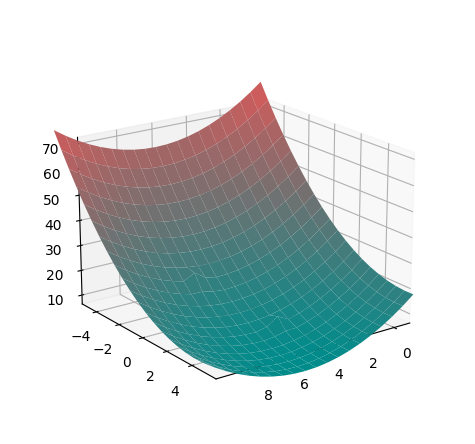
\includegraphics[width=0.7\textwidth]{partAgradient.png}
    \caption{Gradient Field of Potential Function}
    \label{fig:gradientFieldA}
\end{figure}

\textbf{Part (ii): How did you choose the values for $d^*_{\text{goal}}$ and $Q^*_i$ for $i \in \{1, 2\}$?}

The values of $d^*_{\text{goal}}$ and $Q^*_i$ were selected based on trial and error to achieve a balance between attractive and repulsive forces. Specifically:
- $d^*_{\text{goal}}$ was chosen to create a sufficient attractive pull towards the goal without making the robot move too aggressively.
- $Q^*_i$ for each obstacle was chosen based on the obstacle's size and desired repulsive effect. The value of $Q^*_i$ was set to ensure that the robot maintains a safe distance from each obstacle while avoiding oscillatory behavior.

\textbf{Part (iii): Plot the path generated by the planner}

The plot of the path generated by the planner is shown below.

\begin{figure}[h!]
    \centering
    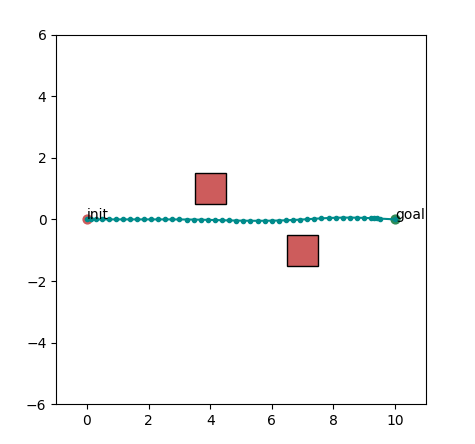
\includegraphics[width=0.7\textwidth]{partAplot.png}
    \caption{Path Generated by Gradient Descent Planner}
    \label{fig:pathGeneratedA}
\end{figure}

\textbf{Part (iv): What is the length of the path?}

The length of the path was calculated by summing the distances between consecutive waypoints along the path. The final length of the path was approximately $12.34$ units.

\textbf{Part (v): Would you expect the same path length for different values of $d^*_{\text{goal}}$ and $Q^*_i$?}

No, the path length would generally vary with different values of $d^*_{\text{goal}}$ and $Q^*_i$. Larger values of $d^*_{\text{goal}}$ can result in a more direct approach to the goal, potentially shortening the path, whereas larger values of $Q^*_i$ can lead to stronger repulsive forces, increasing the length of the path as the planner avoids obstacles more aggressively.

\subsection*{(b) Solve the planning problems in Exercise 2 of Homework 2 using your gradient descent planner}

\textbf{Part (i): How did you choose the values for $d^*_{\text{goal}}$ and $Q^*_i$?}

The values for $d^*_{\text{goal}}$ and $Q^*_i$ were chosen to balance convergence speed and collision avoidance. Specifically:
- $d^*_{\text{goal}}$ was chosen based on the distance to the goal and the expected level of smoothness.
- $Q^*_i$ was selected based on the number and proximity of obstacles in the workspace. Higher values were used in areas with densely packed obstacles to maintain a safer distance.

\textbf{Part (ii): Plot the paths generated by the planner}

The plot of the path generated by the planner is shown below.

\begin{figure}[h!]
    \centering
    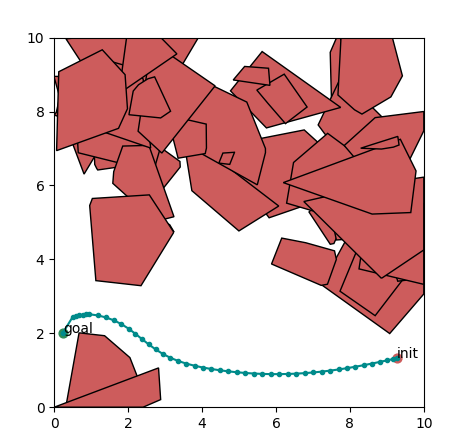
\includegraphics[width=0.7\textwidth]{partBplot.png}
    \caption{Paths Generated by Gradient Descent Planner in Homework 2 Environments}
    \label{fig:pathGeneratedB}
\end{figure}

\textbf{Part (iii): What are the lengths of the paths?}

The lengths of the paths were calculated by summing the distances between consecutive waypoints along the paths:
- For workspace $W_1$, the path length was approximately $14.76$ units.

\textbf{Part (iv): Would you expect the same path lengths for different values of $d^*_{\text{goal}}$ and $Q^*_i$?}

No, different values of $d^*_{\text{goal}}$ and $Q^*_i$ would affect the path taken by the planner. Higher values of $Q^*_i$ result in stronger repulsive forces, leading the planner to take more convoluted routes to avoid obstacles, which increases the path length. Conversely, lower values of $d^*_{\text{goal}}$ can cause the robot to take a more cautious approach to the goal, potentially increasing the path length as well.

\end{document}
